%!TEX root = cscw2018-comic.tex
\section{Discussion}
\label{sec:Discussion}
Here we first summarize our findings from both studies. Then we discuss the effect on Inter-character Distance, the limitations of study, and the design implications of algorithmically synthesizing persuasive messages in abstract comic form.

%need to update this part after the revision of RQ in the introduction
%Our experiment answers RQ-1 affirmatively in that comics are more persuasive than text, with a moderate effect of 0.33. Our answer to RQ-2 is that while the effect of no element is significant, shading and gesture show strong influence, but surprisingly inter-character distance is most effective when distance is large. For RQ-3, we show that negative messages are more influential than positive messages. We have developed a prototypical comic generator (answering RQ-4) that can be used in deploying comic messages.

Our results showed that subjects prefer persuasive messages in comic form over plain text. We found in a persuasive comic, different character's gestures and background shading can influence subjects' perception of the persuasiveness whereas no strong effect was found in inter-character distance. This was consistent with previous research on visual stimulus in persuasion and the benefits of comics in communication. In the second study, we further examined the persuasive power of the abstract comic in real-life decision making. The results clearly demonstrated the persuasive power of abstract comic in nudging people engage pro-social behavioral decisions, i.e. charitable giving. This was consistent with previous research on visual stimulus in persuasion and the benefits of comics in communication.

% followed Our analysis shows that subjects prefer persuasive messages in comic form over plain text. We found in a persuasive comic, different character's gestures and background shading can influence subjects' perception of the persuasiveness whereas no strong effect was found in inter-character distance. This was consistent with previous research on visual stimulus in persuasion and the benefits of comics in communication.
%
\subsection{Inter-Character Distance}
\label{sub:Inter-Character Distance}
There may be two explanations to the odd result that the farthest distance between the two characters was more influential.
% However, previous studies on comics composition suggests the inter-character distance can affect reader's perceived relationship between characters and therefore influence their perception of the persuasive comics.
First, it may be the case that the subjects did not project themselves onto the comic as one of the characters and did not recognize the distance between characters as reflecting closeness of the relationship. For example, a subject may read the comic from a third-person narrative. We looked into some feedbacks from in the pilot study. One participant ($p_1$) mentioned \textit{``I really like the comic I just saw and I feel bad that someone told me ...''} which suggests the subject does think that they are in the comic and having a conversation with someone else. Yet, we don't know if they perceive their relationship with the persuader based on the inter-character distance. A second explanation is that closer inter-character distance causes a cluttered visual composition and thus the subjects perceive these comics as less visually pleasing.

% \subsection{Comics with Color}
% \begin{figure}[t]
%  \centering
%  \begin{tabular}{ccc}
%   \subfloat[Colored Text]{\label{figur:3o}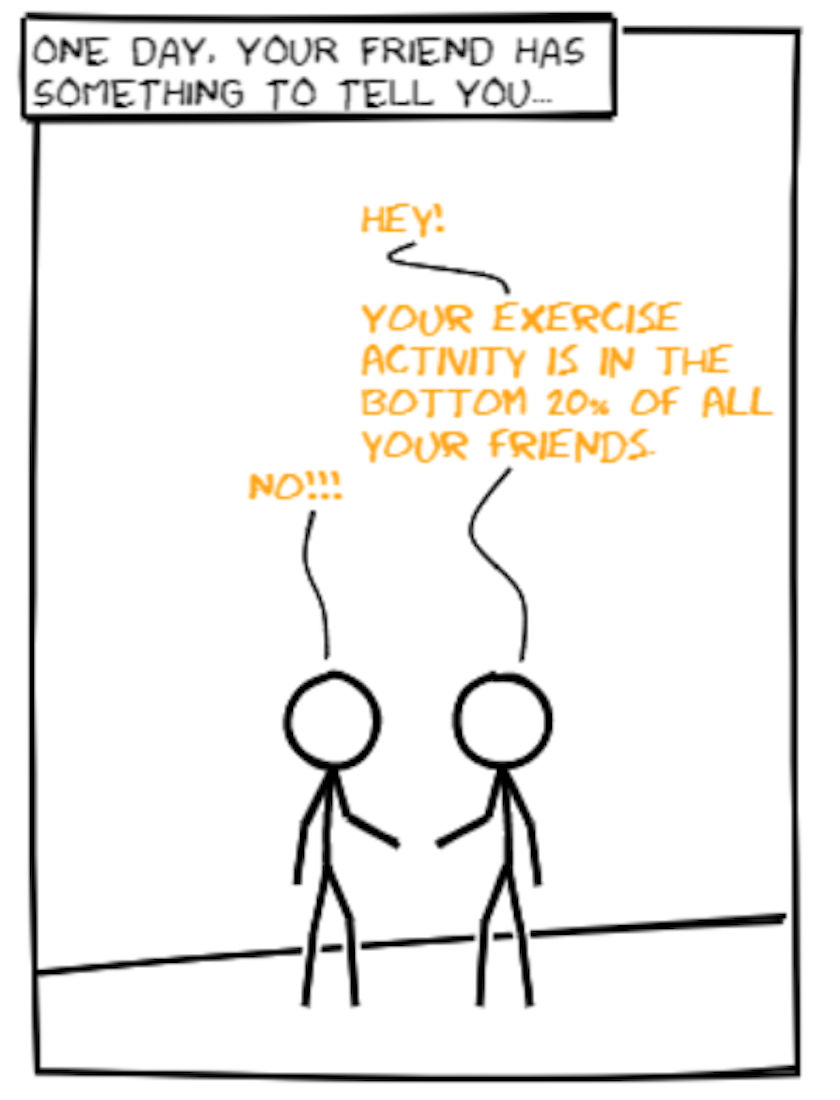
\includegraphics[width = 0.27\columnwidth]{figures/o1}} &
%   \subfloat[Colored Ground Line]{\label{figur:31}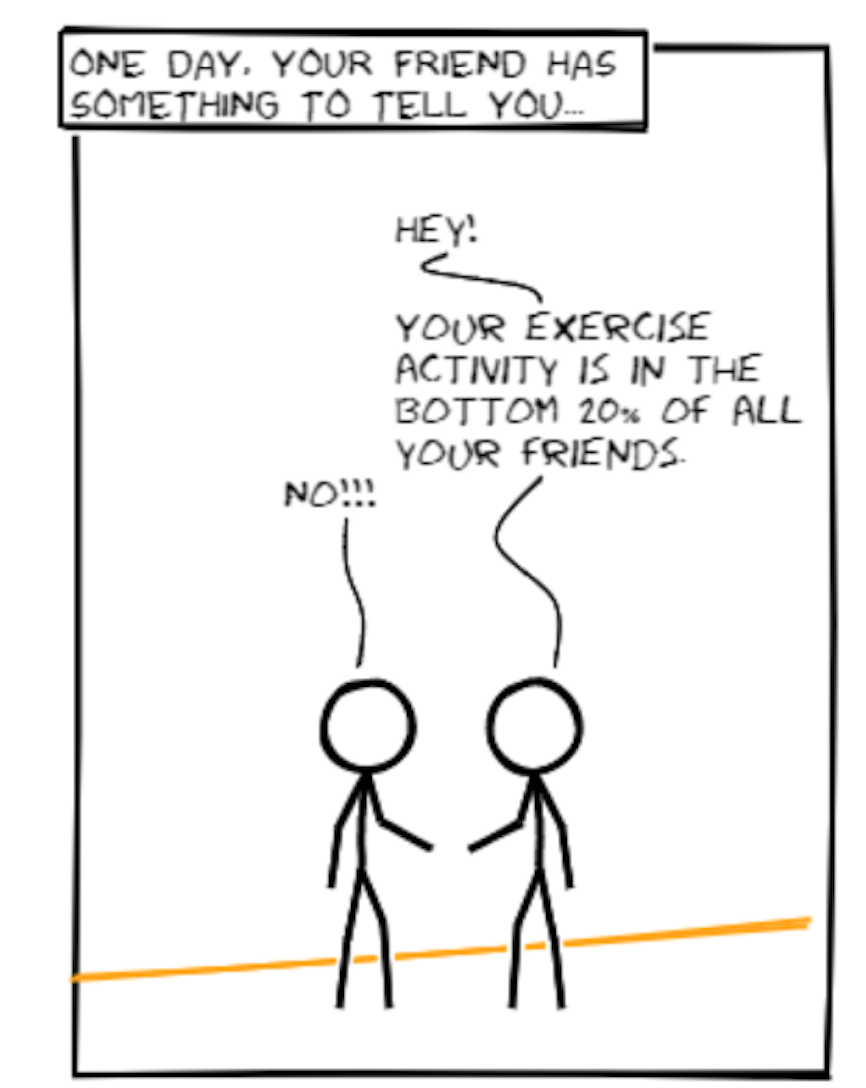
\includegraphics[width = 0.27 \columnwidth]{figures/o2}}      &
%   \subfloat[Colored Figure]{\label{figur:32}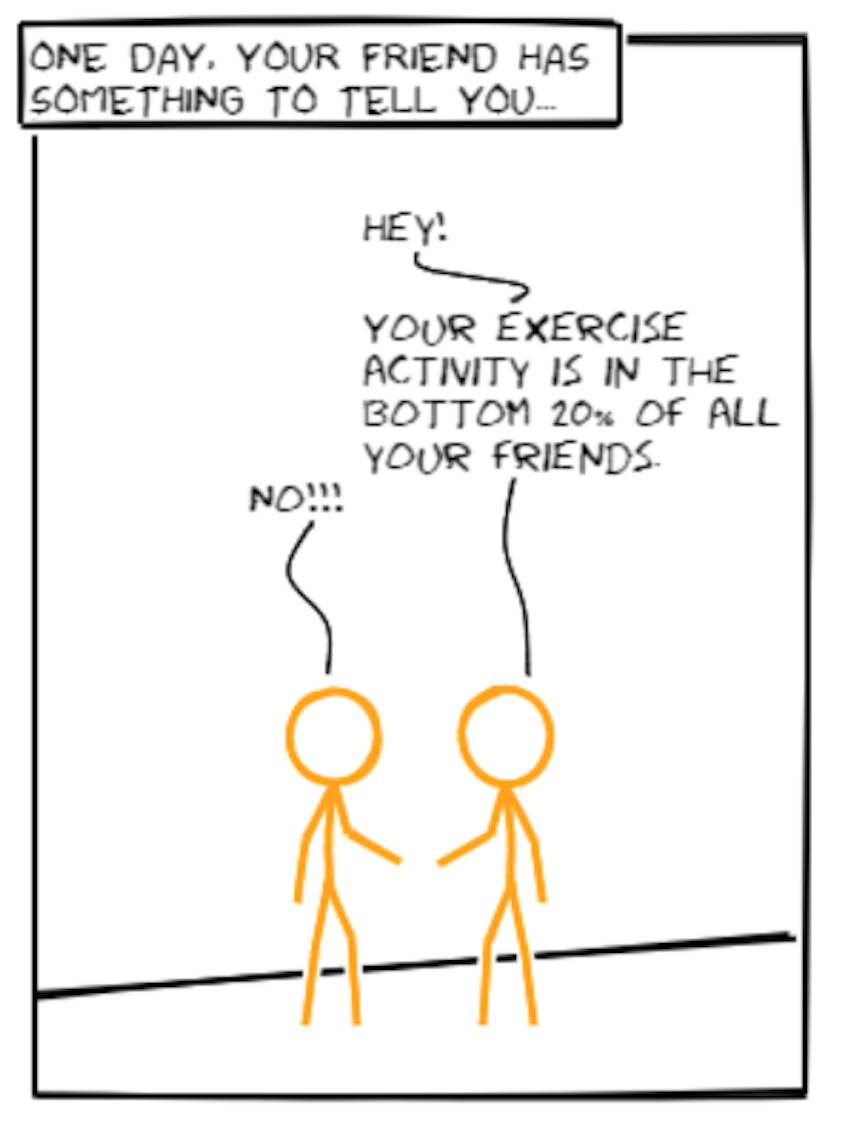
\includegraphics[width = 0.27 \columnwidth]{figures/o3}}\\
%  \end{tabular}
%  \caption{Colored different elements in a comic}
%  \label{figur:color}
% \end{figure}
%
% Our model suggests the background shading in a persuasive comic affects its persuasive power which makes us wonder the role of color as previous studies suggest the usage of color communicates the emotional intensity similar to the background shading. We ran a small scale study comparing the perceived persuasiveness between black-white comics in our study and their corresponding colored version,see figure~\ref{figur:color}. With 60 participants from the Mechanical Turk,  we found using an identical hierarchical Bayesian formulation that our subjects perceive colored version as more persuasive and there is potential interaction effect between negative-positive framing and different colors (see~\Cref{fig:color-experiment-effect}). We plan to run larger experiments that include color and study the interaction with framing and other elements.
%
% \begin{figure}
%  \subfloat[The mean effect and the effect size with color\label{subfig-1:color-mean-effect}]{%
%   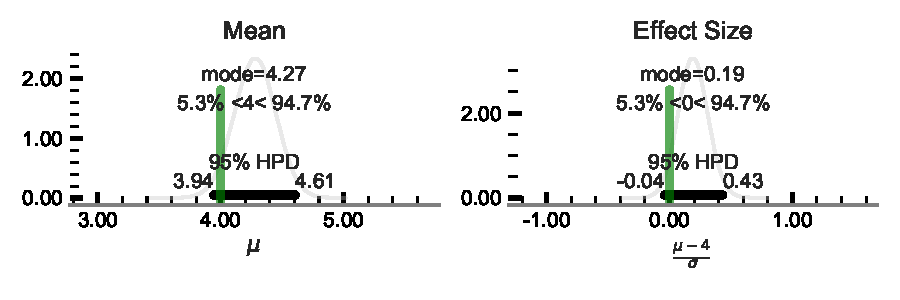
\includegraphics[width=0.6\textwidth]{./hari-code/factors_mean_effect_color-no-interaction.pdf}
%   } \hfill
%  \subfloat[Color contrast\label{subfig-2:color-contrast}]{%
%   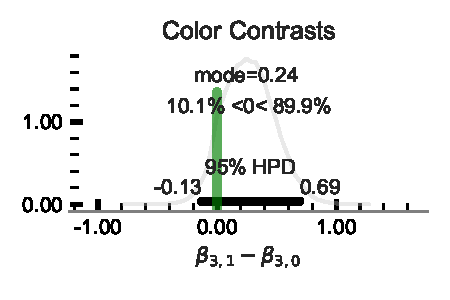
\includegraphics[width=0.33\textwidth]{./hari-code/factors_color_contrasts_color-no-interaction.pdf}
%  }
%  \caption{~\Cref{subfig-1:color-mean-effect} shows the High Posterior Density (HPD) intervals for the mean response $\mu$ and effect sizes $\sigma_y$ in the presence of color. HPD represent the region with 95\% of the density. Notice that the HPD interval for $\mu$ is $[3.94, 4.27]$ and includes a ROPE of $[4\pm 0.1]$ (the interval includes 4, the neutral response value). Thus while there no significant effect, we note that nearly 94\% of the HPD lies to the right of 0. The figure for effect size shows a small effect with mode $0.19$; since the HPD interval $[-0.04, 0.43]$ includes a ROPE of $[0\pm 0.1]$, there is no significant effect.~\Cref{subfig-2:color-contrast} shows the contrasts between the use of the two colors. The modal value is $0.24$, but since the HPD interval $[-0.13, 0.69]$ overlaps with 0, there is no appreciable effect (but notice that 89\% of the density lies in the region greater than 0.)}
%  \label{fig:color-experiment-effect}
% \end{figure}


\subsection{Limitations}
Our current work has several limitations.
\begin{description}
 \item[No interaction effects in model]: Our model does not include any interaction effects. This is by design, since we have 54 experimental conditions making the any analysis interaction effects difficult with our small observational study. The raw data suggests an interaction between shading and gesture, but given our limited dataset, there is little point in modeling this interaction. We plan to study interaction effects in future studies by limiting the number of main predictor conditions.
 \item[Generalizability]:  Although our second study asked participants to make decision with cost, the decision domain is limited to only one scenario, charitable giving. Future studies were needed to see if the persuasive power of abstract comics can generalize to multiple domains

 \item[Ecological Validity:] There is a ligitimate question if our experiment on Amazon Mechanical Turk has ecological validity. In real life, a lot of factors may affect people's decision, such as where they are and who they are interacting with. Those factors may interact with the abstract comic's persuasiveness. Large scale field study is needed to demonstrate how the abstract comic can persuade in the real-life decision making and what will affect its persuasiveness. 
 %Since we ask the subjects (who may lack interest in exercise) to evaluate persuasiveness when the topic is on exercise. Notice that our goal is not to persuade experimental subjects to exercise more, but to evaluate if the comic is a more persuasive form of communication of a statistical fact. We should expect---since we don't know if the subjects are interested in exercise---an increase in the variance in the estimates of the parameters (in particular,  $\sigma_y$). Despite this, the analysis shows a significant affirmative result for RQ-1.
 \item[Appropriate gestures]: The authors determined gestures used by the characters in the experiment through trial and error. It may be useful to examine dance theory as well as work on designing sign languages.
\end{description}
 % \item[Single Panel]: Our experiment limits our comics to a single panel which hinders one of the most fascinating aspect of comics---storytelling. Comparing to the comic strip, single panel comics find it harder to show the dynamic among characters.
\subsection{Design Implications and Future Work}
Taking the advantage of data driven methods, the abstract-comic can better persuade. In our study, we know comic elements can deliver the persuasiveness differently. Therefore, to maximize the persuasive power, future research on computational persuasion should leverage receiver's personal model to construct the persuasive abstract comics with elements best fit to the persuadee.
